\documentclass{article}
\usepackage{geometry}
\usepackage{flafter}
\usepackage{float}
\geometry{letterpaper, portrait, margin=1in}

\usepackage{hyperref}
\hypersetup{
    colorlinks=true,
    linkcolor=black,
    filecolor=magenta,
    urlcolor=blue,
}

\usepackage{graphicx}
\graphicspath{ {images/} }

\usepackage{tcolorbox}
\usepackage{textcomp}
\usepackage{gensymb}
\usepackage{indentfirst}

\newcommand{\ans}{$\rule{1.5cm}{0.15mm}$}

\title{RoboJackets Electrical Training Week 2 Lab Guide}
\author{Asha Bhandarkar}
\date{\today\\v1.0}

\begin{document}
\maketitle{}
\setcounter{tocdepth}{2}
\tableofcontents
\pagebreak

%Everything below is for you to edit. Code above sets up the general formatting for the document

\section{Background}
In the Week 2 Electrical Training lecture, you learned about PCBs, EAGLE, Libraries, and Parts. In RoboJackets, PCB design is an integral part of our autonomous teams' electrical stack, thus if you are interested in PCB development for RoboJackets and hardware design in general, learning how to use EAGLE is essential.

In today's lab we will be focusing on making a part in EAGLE and adding it to a library. Oftentimes, we have to make or modify a part as a CAD file for it is not always available or it is insufficient. 

\section{Objective}
\subsection{Install EAGLE and other Software}
\begin{itemize}
    \item If you have not already installed EAGLE, please install it from \href{https://www.autodesk.com/education/free-software/eagle}{here}. Make sure to install the education version to get all of the features of EAGLE. With this link, create an education account for Autodesk (in Week 1 you already did this step for setting up TinkerCAD). Then navigate to your profile and look at "All Products and Services". There, you should see a download for EAGLE Premium available.
    \item If using Mac/Windows follow instructions to install Github Desktop from \href{https://docs.github.com/en/desktop/getting-started-with-github-desktop/installing-github-desktop}{here}. If you are familiar with Git in terminal you can use this instead and that can be installed \href{https://git-scm.com/book/en/v2/Getting-Started-Installing-Git}{here}. If you are using Linux you will need to use Git in terminal. 
    \item Clone the repository eagle-libraries \href{https://github.com/RoboJackets/eagle-libraries}{here} and configure your EAGLE setup using the instructions in the README. Also clone the electrical-training repository \href{https://github.com/RoboJackets/electrical-training/tree/master}{here}
    \item Note: If you are having trouble with any of these steps please let an instructor know
\end{itemize}
\subsection{Create a Part in EAGLE}
\begin{itemize}
    \item Create a new EAGLE Library called "week2" by going to the control panel File $\rightarrow$ New $\rightarrow$ Library. Add a symbol, footprint, and device for a 3D Hall Sensor. Detailed steps on how to do this are outlined in the Guided Lab section of this document.
\end{itemize}


\section{Materials}
\begin{itemize}
	\item \href{https://www.autodesk.com/education/free-software/eagle}{EAGLE} (with education license)
	\item \href{https://docs.github.com/en/desktop/getting-started-with-github-desktop/installing-github-desktop}{Github Desktop} or \href{https://git-scm.com/book/en/v2/Getting-Started-Installing-Git}{Git} in Terminal
	\item Cloned repositories \href{https://github.com/RoboJackets/eagle-libraries}{\texttt{eagle-libraries}} and \href{https://github.com/RoboJackets/electrical-training/tree/master}{\texttt{electrical-training}}
	\item \href{https://media.digikey.com/pdf/Data%20Sheets/Infineon%20PDFs/TLE493D-A2B6_V1.3_4-9-19.pdf}{3D Hall Sensor Datasheet} (TLE493DA2B6HTSA1)
	\item Recommended: An external mouse
\end{itemize}

\section{Relevant Information}
\subsection{Reading a Pin Configuration}
When making parts in EAGLE, the component's datasheet will be your best friend. It should tell you all the information you need to create the symbol and footprint. To make a symbol, you will often look for a pin configuration (also called a pinout) to see what individual pins/pads on a part actually do. For our use case, page 5 of the datasheet gives the pin configuration which is also pictured below. Usually the pins are numbered and their names and descriptions are given below. These are usually the same names you will give your pins in your symbol. For example, when we make the symbol, we will have a pin called SDA/INT to represent the function of pin 1 of the sensor.
\begin{figure}[ht]
    \center
	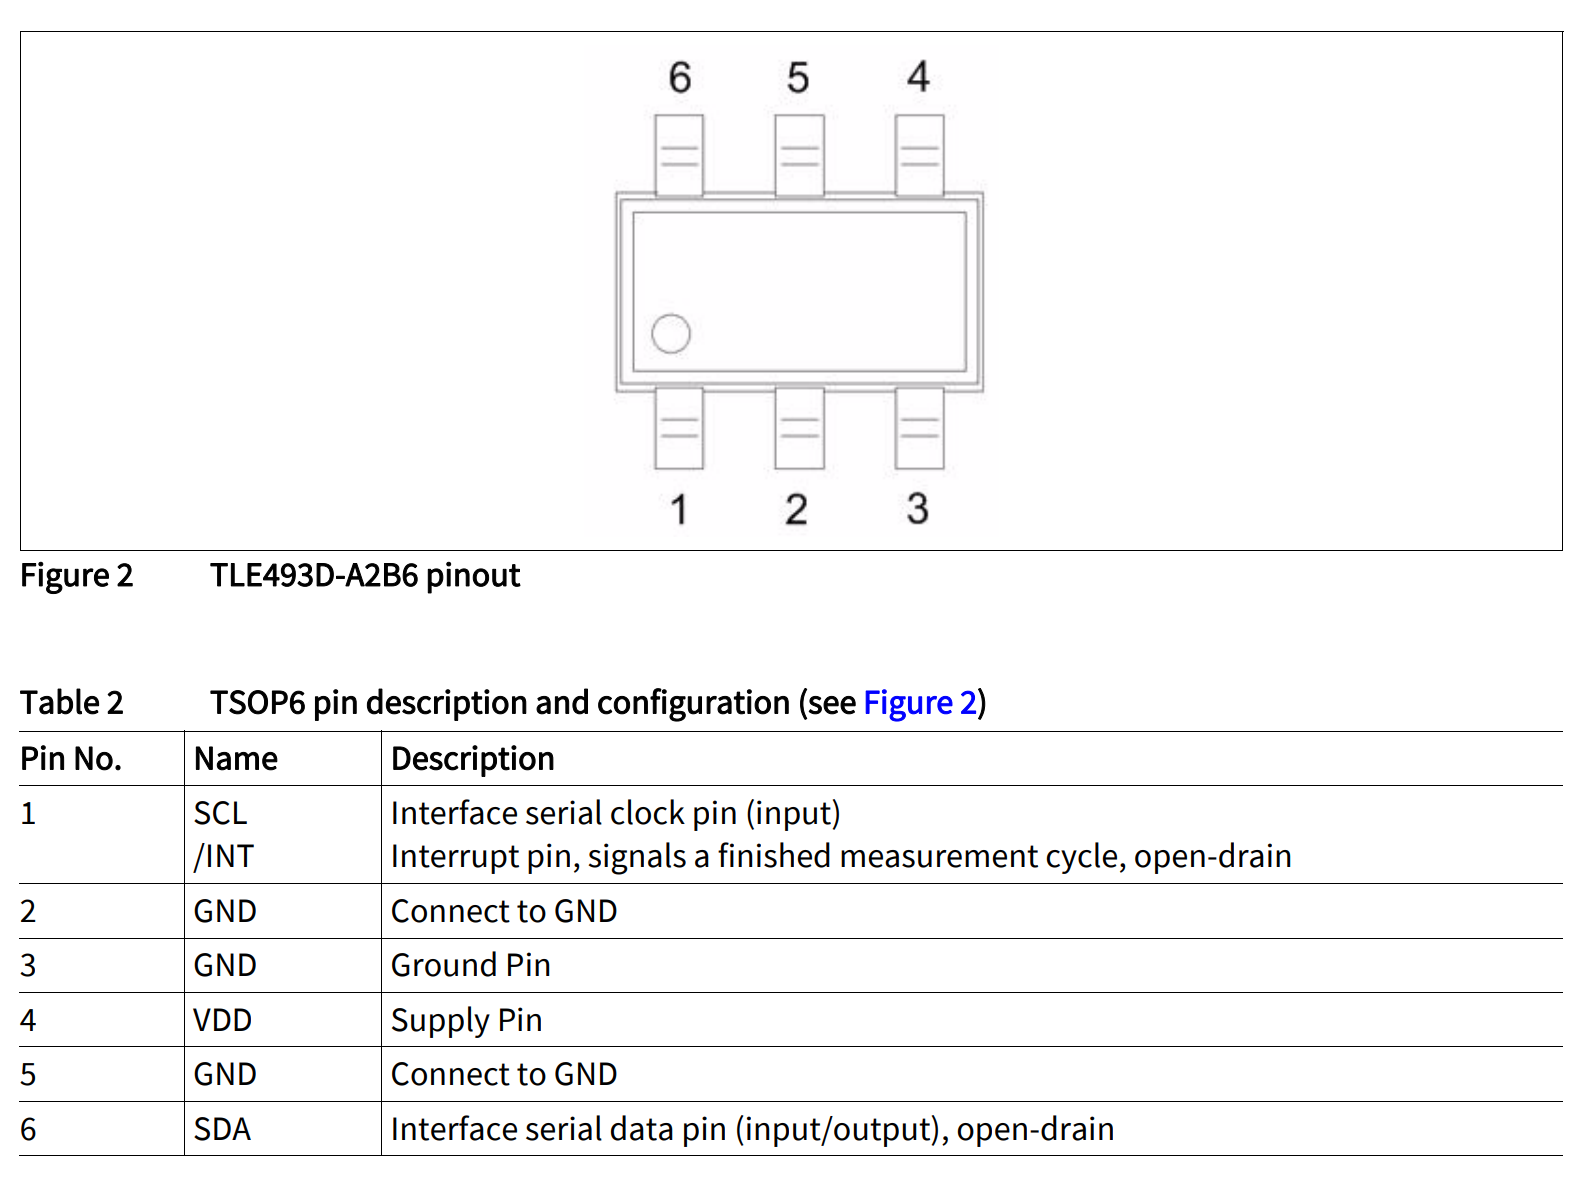
\includegraphics[width=0.9\textwidth, keepaspectratio]{images/pinconfig.png}
	\caption{Pin configuration for sensor}
	\label{fig:pinconfig}
\end{figure}

\subsection{Reading Package Information}
To make the footprint, we will look for the package information. Generally this will look like a drawing of the chip with several measurements, including basic length and width, size of pins, and the distance between pins. For this component, page 17 and 18 has information about the package. Figure 8 from that datasheet is included below as it contains sufficient information to make the footprint. 
\begin{figure}[ht]
    \center
	
\includegraphics[width=0.8\textwidth, keepaspectratio]{images/package.png}
	\caption{Package for sensor} 
	\label{fig:package}
\end{figure}

\section{Guided Lab}
\subsection{Creating Symbol}
\subsubsection{Adding to Library}
\begin{itemize}
    \item Click "Add Symbol" and type in the specific part number for this sensor (TLE493DA2B6HTSA1)
\end{itemize}
\subsubsection{Creating and Defining Pins}
\begin{itemize}
    \item Check grid to make sure the dimensions are correct (0.1 inch Size, 0.01 Alt) by clicking the grid icon in the top left.
    \item Based on the pin configuration there are 4 different types of pins - the SCL/INT, SDA, VDD, and GND pins. The chip has multiple GND pins, but for the symbol these can be grouped together.
    \item Add 4 pins with those names to your grid using the "Add Pin" button on the left menu. Set the direction of the pins to passive (check the properties of the pin). This is done versus being more specific to avoid unnecessary design rule check (DRC) errors.
\end{itemize}
\subsubsection{Draw Outline}
\begin{itemize}
    \item Using the line tool located on the left menu, create a box, centered on the origin (the cross). Arrange the pins in a way that they attach to this box. Using the grid to create equal spacing is a good practice. 
\end{itemize}
\subsubsection{Adding Name and Value}
\begin{itemize}
    \item Switch your layer to \texttt{95 Names} and by using the text feature type \texttt{>NAME} and place it in the upper left corner of your part. Use 0.07 vector font. The layer tool is a dropdown on the top bar. The text tool is on the left and the font can be changed on the top bar.
    \item Switch your later to \texttt{96 Values} and using the same process as above type \texttt{>VALUE} and place it in the bottom left corner of your part
\end{itemize}

\begin{figure}[h]
    \center
	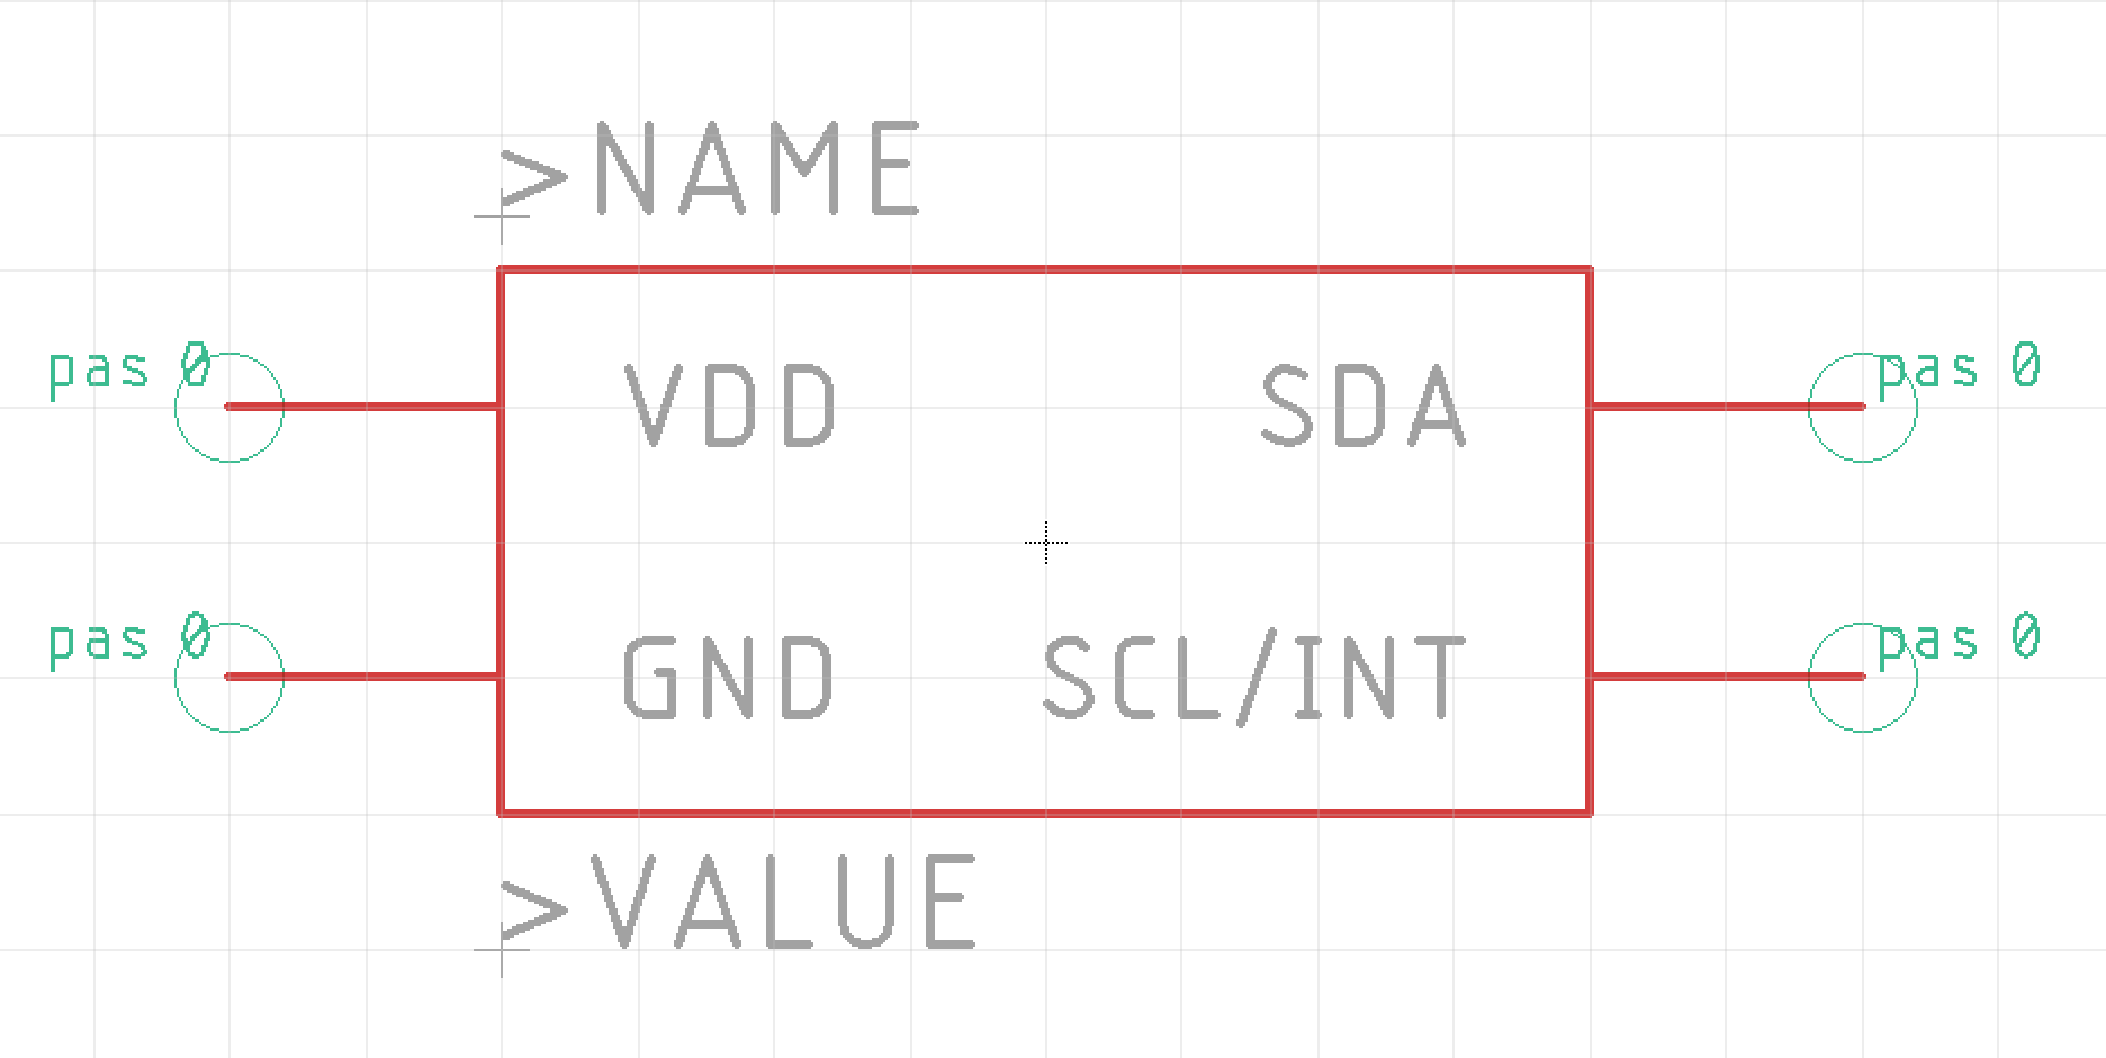
\includegraphics[width=0.7\textwidth, keepaspectratio]{images/symbol.png}
	\caption{Finished symbol for the 3D Hall Sensor}
	\label{fig:symbol}
\end{figure}


\subsection{Creating Footprint}
\subsubsection{Adding to Library}
\begin{itemize}
    \item To get back to the main library menu, go to Library $\rightarrow$ Table of Contents
    \item Click "Add Footprint" and type in the package name which can be found on page 17 of the datasheet (TSOP6).
\end{itemize}
\subsubsection{Creating SMD Pads}
\begin{itemize}
    \item For making the footprint, keep the cross in the middle of the footprint so calculations for placement are easier
    \item Check grid to make sure dimensions are correct (1 mm Size, 0.1 mm Alt)
    \item Begin by adding a "SMD" on the \texttt{1 Top} layer. Specify the dimensions of the SMD and it's location by accessing its properties. The numbers for the dimensions and location can be figured out from the diagram on page 17 of the datasheet which is also included earlier in this lab document. The position refers to the x and y coordinates on your grid. The SMD size can be adjusted using either the dropdown or by typing in your own values. The SMD tool is on the left menu.
    \item Continue this process for the remaining SMDs. As you add SMDs, you will notice that they are automatically numbered. It is useful to match this numbering to what is in the pin configuration as it makes making the device easier
\end{itemize}
\subsubsection{Adding Silkscreen}
\begin{itemize}
    \item Switch your layer to \texttt{21 tPlace} and add a box around the part, on the inside of the pins using the line tool. Make sure your line does not cover the SMD pads. You can easily adjust this by using the move tool while pressing the \texttt{Alt} key which allows you to use the smaller 0.1 mm grid we set earlier. 
    \item When soldering, it is nice to know the directional of the chip. Thus, it is a common practice to add a dot near pin 1. You can do this by using the polygon tool to draw a small circle, adjusting is size as appropriate, and placing it near SMD pad 1. The polygon tool is located in the left menu. 
\end{itemize}
\subsubsection{Adding Keep Out Boundary}
\begin{itemize}
    \item To make sure that parts do not overlap later when we route them, it is useful to set a boundary around the entire part
    \item Switch your layer to \texttt{39 tKeepout} layer and add a 0.1 mm width line around the entire part. Like earlier, you can make this more precise by using \texttt{Alt}
\end{itemize}
\subsubsection{Adding Name and Value}
\begin{itemize}
    \item Follow the same process as you did for the symbol to add the \texttt{>NAME} and \texttt{>VALUE} to your footprint. Use the \texttt{25 tNames} layer and the \texttt{27 tValues} layer
\end{itemize}
\begin{figure}[H]
    \center
	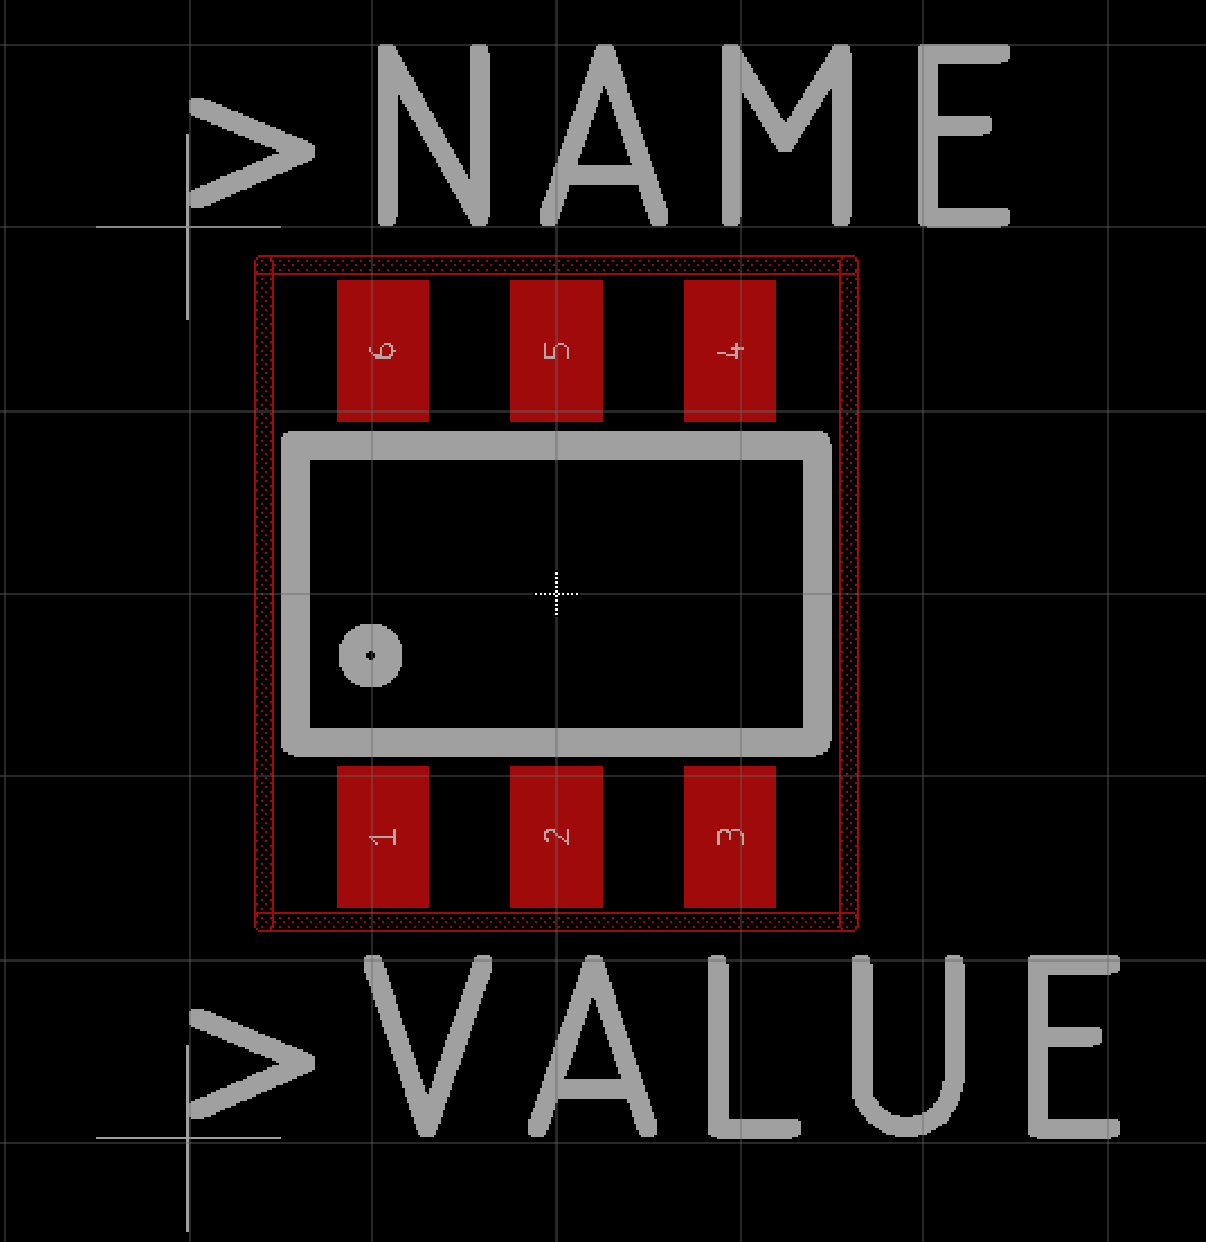
\includegraphics[width=0.4\textwidth, keepaspectratio]{images/footprint.png}
	\caption{Finished footprint for the 3D Hall Sensor}
	\label{fig:footprint}
\end{figure}


\subsection{Creating Device}
\subsubsection{Adding to Library}
\begin{itemize}
    \item Click "Add Device" and type in the specific part number for this sensor (TLE493DA2B6HTSA1)
\end{itemize}
\subsubsection{Adding Symbol and Footprint}
\begin{itemize}
    \item To add the symbol, use the "Add Part" button located in the left menu and center in on the cross
    \item To add the footprint, click "New" in the bottom right and then "Add local package" to find the footprint we made earlier
\end{itemize}
\subsubsection{Connecting Symbol and Footprint}
\begin{itemize}
    \item Now we will connect the connections we made on the symbol to the corresponding pads on the footprint, using connect and our pin configuration from earlier 
    \item For example, let us connect pin 1 from our configuration. Based on this diagram, it corresponds to SCL/INT pin on the symbol and pad 1 on the footprint. You can select these two and connect them. They should now appear on the "Connection" part of the panel
    \item What do we do if we have a pin that corresponds to multiple pads as is the case with GND? In this case you can connect the first pad to the pin and then use "Append" for the rest
    \item After you have completed this process for all the pins and pads you have connected your symbol and footprint!
\end{itemize}
\subsubsection{Adding Prefix}
\begin{itemize}
    \item Now we will add the prefix (located in the bottom right) which will later show up in the name of the part when used in a schematic and board. Here we will select "U" since we are dealing with an IC. Details on prefixes are included in the RJ Style Guide.
\end{itemize}
\subsubsection{Adding Attribute and Description}
\begin{itemize}
    \item Now we are going to add details to the part that make it easier when we go to order the board or to track down a specific part
    \item In the attribute section add a new attribute that named DKPN (Digikey Part Number, Digikey is the distributor we order electrical components from) and enter the part number given on the Digikey website \href{https://www.digikey.com/product-detail/en/infineon-technologies/TLE493DA2B6HTSA1/TLE493DA2B6HTSA1CT-ND/9808573}{here}
    \item In the description, add a link to the datasheet and give a one sentence description of this part. Finally keep the value "Off" for this part. When doing passive components (resistors, capacitors) you will want to turn this on.
\end{itemize}
\begin{figure}[H]
    \center
	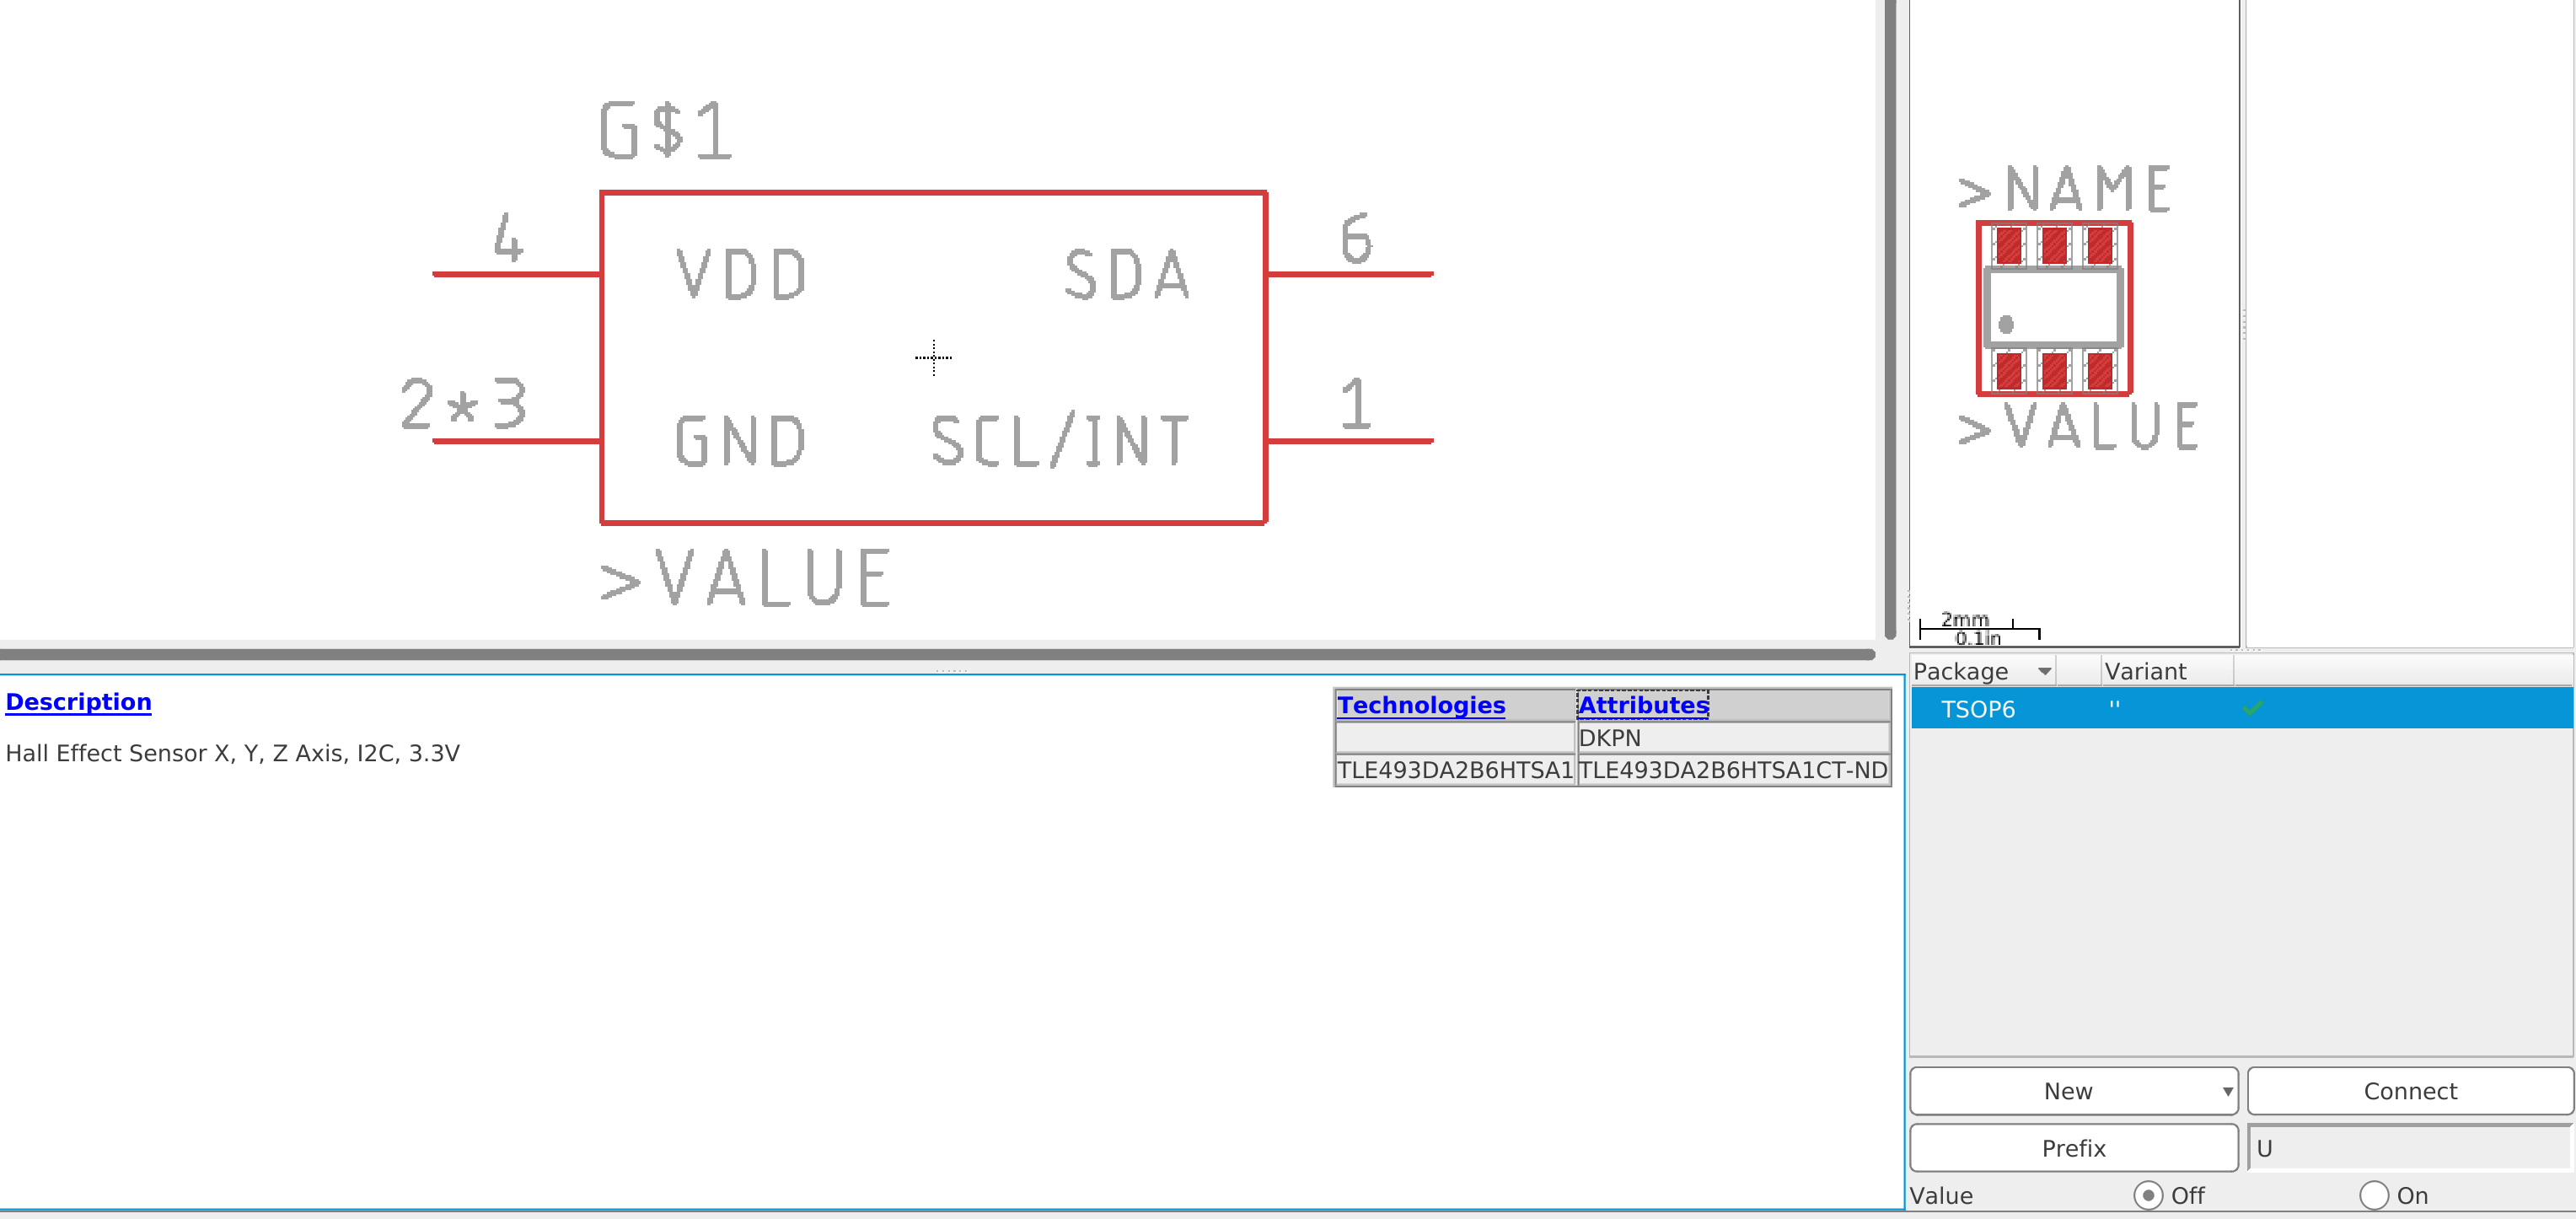
\includegraphics[width=0.8\textwidth, keepaspectratio]{images/device.png}
	\caption{Finished device for the 3D Hall Sensor}
	\label{fig:device}
\end{figure}

You have now created a part! In next week's lab you will actually be using parts and you will learn how to include them on a schematic



\section{Troubleshooting}
For any problems with your EAGLE or GitHub Desktop/Git installations please reach out to an instructor who can help with your specific issue.

Below are some EAGLE Resources you will find useful as you complete this lab and in general during your time in RoboJackets
\begin{itemize}
    \item \href{https://wiki.robojackets.org/EAGLE_Style_Guide}{RoboJackets Style Guide} - Details what is needed in a part, schematic, and board in terms of setting and style.
    \item \href{https://github.com/RoboJackets/electrical-training/blob/master/references/eagle_training_guide/eagle_guide.pdf}{EAGLE Training Guide} - A comphrehensive guide on how to do common things in EAGLE
    \item \href{https://github.com/RoboJackets/electrical-training/blob/master/references/eagle_cheat_sheet/eagle_cheat_sheet.pdf}{EAGLE Cheat Sheet} - A guide to all of the buttons that are available to you on the schematic and board layout views which have some overall with the symbol, footprint, and device windows
    \item \href{https://www.youtube.com/watch?v=ayiXpakBtsM&list=PL1R5gSylLha2iQ7e9mwiXJDY2RXoM8HxK&index=2}{RoboJackets Part and Libraries Video} - contain information and walks through how to make a part
\end{itemize}


\end{document}